\documentclass[12pt, class=report, crop=false]{standalone}
\usepackage{ba_thesis}

\begin{document}

\chapter{Numerical Methods and Particle in Cell Simulations}%
\label{chap:numerical-methods}

The domain of numerical simulations for laser-plasma interaction is incredibly expansive, with many approaches one can choose from, like numerically solving the Vlasov equation or using Particle-in-cell methods, and many ways to implement and optimize them. I will restrict in this thesis to the second option.

Even so, there are two key integration schemes that sit at the core of a Particle-in-cell software, the Maxwell solver and the particle pusher. In this chapter I aim to analyze in detail the most used schemes and their propeties and eventually give a bird's eye view of the currently available PIC codes out there and the implementation choices they've made.

\section{The Relevant Equations}

Particle-in-cell codes are nowadays the most popular popular tool for simulating plasma systems. One of the best references for what they are, how they work and how reliable the results are is the book by~\cite{birdsallPlasmaPhysicsComputer1995}, which describes the main numerical methods used and some of their properties. However, Particle-in-cell codes have evolved greatly in the last two decades and new techniques and optimizations have been produced and even put in practice. Even so, with the exception of quasistatic codes, they are still involved in solving the same physical equations. As such, it is useful for anyone interested in working with such software to know and understand the principles behind.

In general, PIC codes have four main componets:
\begin{enumerate}
  \item A Maxwell solver which propagates the Maxwell equations (which are relativistic invariant by themselves) in time and space on the grid
  \begin{subequations}
    \begin{align}
    \div{\vb{E}} & = \frac{\rho}{\varepsilon_0} \\
    \div{\vb{B}} & = 0 \\
    \curl{\vb{E}} & = - \pdv{\vb{B}}{t} \\
    \curl{\vb{B}} & = \mu_0 \vb{j} + \frac{1}{c^2} \pdv{\vb{E}}{t} \,;
    \end{align}
  \end{subequations}
  \item A field gatherer that interpolates the electromagnetic field at the particle positions on the grid;
  \item A particle pusher that advances the positions and velocities of each particle under the action of the Lorentz force (which we will write in its relativistic form)
  \begin{subequations}
    \begin{align}
      \label{eq:NL}
      \dv{\vb{p_\alpha}}{t} = q_\alpha \left(\vb{E}+\frac{\vb{p_\alpha}}{m_\alpha \gamma_\alpha} \cp \vb{B} \right)\\
      \gamma_\alpha = \sqrt{1+\left(\frac{\vb{p_\alpha}}{m_\alpha c}\right)^2}\,,
    \end{align}
  \end{subequations}
  where \(\alpha\) indexes each particle;
  \item Acurrent and charge depositor which computes the current and charge densities on the grid by interpolating the particle distributions.
\end{enumerate}

The main appeal of this approach is its self-consistency. That is, the total fields used are both those that are part of the electromagnetic waves that are introduced in the system (in general laser beams) and those generated by the charged particles that compose the plasma. As such we also include the long range Coulombian interaction between particles. The short range interaction, namely collisions between particles, is by default neglected since we usually simulate rarefied plasmas, but many codes now come with additional routines that include these processes. Additional routines are now developed with the advent of the high intensity laser technologies because at the corresponding energies reached by the particles quantum electrodynamical effects become relevant. Although there are quite a few PIC codes that include QED routines, there is still a long way untill these algorithms reach the efficiency and stability that of those four main ones described above. As such, the implementation of QED effects in numerical plasma simulations is currently a hot research topic.

It is mandatory to mention that while the four steps above outline a microscopic model, PIC simulations are not completely microscopic due to technological limitations regarding computing power. Instead of working with one virtual particle for one real particle, it is customary to use macro-particles. A macro-particle represents many particles of the same species (from \(10^6\) to \(10^11\) depending on the propeties of our plasma) moving colectively. These particles are obviously not localized at a single point, but rather they have a shape function attached to them to make the derivation of currents and charge densities more consistent. For a long time the use of macro-particles was not supported by argument and was a source of criticism towards PIC methods. The defense was built only on the excuse of that the simulations give very accurate statistical results. Things are different nowadays. We can now explain (quite easily in fact) that the macro-particles themselves can be interpreted a statistical ensamble of real particles. The secret lies in the Vlasov equation.

\subsection{The Connection with the Vlasov Equation}

Let us revisit the Vlasov equation, which we derived in~\cref{sec:Vlasov}

\begin{equation}
  \pdv{\rho}{t} + \vb{f}\vdot\pdv{\rho}{\vb{p}} + \vb{v}\vdot\pdv{\rho}{\vb{r}} = 0\,,
\end{equation}
where \(\rho\) was the distribution function that describes the entire system of particles, \(\vb{p}=(\vb{p_1}, \vb{p_2},\dots )\) and \(\vb{v}=(\vb{v_1}, \vb{v_2},\dots )\), \(\vb{r}=(\vb{r_1}, \vb{r_2},\dots )\) the momenta, the velocities, and the positions of the particles, and \(\vb{f}=(\vb{f_1}, \vb{f_2},\dots )\) the forces acting on each particle.

The main argument in the following discussion is a relativistic upgrade of the one in~\cite{liuHighPowerLaserPlasmaInteraction2020}. For consistency with the equations we outlined for the PIC method, I rewrite this equation in its relativistic form and considering all forces to be of the Lorentz type

\begin{equation}
  \pdv{\rho}{t} + \sum_\alpha \left[ q_\alpha \left(\vb{E_\alpha}+\frac{\vb{p_\alpha}}{m_\alpha \gamma_\alpha} \cp \vb{B_\alpha} \right) \pdv{\rho}{\vb{p_\alpha}} +  \frac{\vb{p_\alpha}}{m_\alpha \gamma_\alpha} \pdv{\rho}{\vb{r_\alpha}}\right] =0\,,
\end{equation}
where \(\alpha\) indexes all the particles in the system and the fields \(E_\alpha\) and \(B_\alpha\) are to be computed at the position of particle \(\alpha\).

The key insight now is that imposing that the particles move under the Newton-Lorentz~\cref{eq:NL} implies having a stationary solution for the distribution function. That is, the equations

\begin{subequations}
  \label{eq:boris1}
  \begin{align}
    \dv{\vb{p_\alpha}}{t} = q_\alpha \left(\vb{E}+\frac{\vb{p_\alpha}}{m_\alpha \gamma_\alpha} \cp \vb{B} \right)\\
    \dv{\vb{r_\alpha}}{t} = \frac{\vb{p_\alpha}}{m_\alpha \gamma_\alpha}\,,
  \end{align}
\end{subequations}
reduce the Vlasov equation as follows

\begin{equation}
  \pdv{\rho}{t} + \sum_\alpha \left( \pdv{\rho}{\vb{p_\alpha}}\dv{\vb{p_\alpha}}{t} + \pdv{\rho}{\vb{r_\alpha}} \dv{\vb{r_\alpha}}{t} \right) = \dv{\rho}{t} = 0 \,.
\end{equation}

Of course this is not an equivalency. While~\cref{eq:boris1} implies that the distribution function of the entire system is stationary, the reverse is not true, unless we do a rough approximation and suppose that the total distribution can be separated in a sum of independent single particle distribution functions. By employing this latter approximation we would unavoidably neglect some intrinsic interactions that take place in our system. Nonetheless, this problem does not affect the validity of our Particle-in-cell method. The thing is that while~\cref{eq:boris1} doesn't describe all the complete stationary solution of the Vlasov equation, it still describes at least one particular stationary solution. Working with superparticles is like studying the evolution of an ensable of these solutions. Thus, by including a relevant (yet not large enough to give unreasonable simulation times) number of superparticles we obtain a statistically realistic solution. Some even call PIC a Monte-Carlo method because of this.

The reverse approach is used in numerical studies of plasma physics using Vlasov codes (VC). These approaches simply try to solve the Vlasov equation as it is in order to obtain exact solutions (exact up to numerical errors). If one has the total distribution function then every statistical piece of information about the system is known. Some basics about how this can be achieved and computational optimization can be found in~\cite{silinVlasovcodeSimulationsCollisionless}. However, directly solving such a big solution with a number of variables proportional to the real number of particles in the system takes a lot of time if we try to simulate realistically sized systems.

An approach based on the splitting of the distribution function is not completely flawed. One can try to get closer to reality by using a better approximation by expanding the total distribution in a series that contains single-particle terms, two-particle terms, and so on. While it is true that this improves the solutions greatly, the cost in computation time is equally great and much refinement would have to be done.

The presentation so far should not give the reader the impression that PIC is the supperior approach. In fact, numerical heating is a common problem of PIC codes and the stability conditions for the simulations are quite restrictive, which together with the computational limitations reduce the amount of experiments you can run. An easy to follow rought sketch of the trade off between PIC and VC and a discussion on when is one better than the other is found in~\cite{bertrandVlasovModelsLaser2005}.

\section{Numerical Methods}

In this section I aim to summarize the basic theory in the area of numerical methods that would be required to understand the schemes that comprise PIC codes and the problmes they pose. The presentation will be a short review of the concepts developed in the second chapter of the book by~\cite{leimkuhlerSimulatingHamiltonianDynamics2004}.

\subsection{Introduction to Numerical Methods for Solving Differential Equations}

We aim to understand how to find numerical solutions for a system of \(k\) ordinary differential equations with initial condition

\begin{equation}
  \label{eq:ODE}
  \dv{\vb{u}}{t} = \vb{f}(\vb{u}),\; \vb{u}(t_0) = \vb{u_0} \in \mathbb{R}^k\,,
\end{equation}
where \(t_0\) is the initial time, \(\vb{u_0}\) is the initial value of our solution and \(\vb{f}\) is a function that relates the elements in the solution vector. We can always set the time such that we have \(t_0=0\) for simplicity.

We usually refer to the solution \(\vb{u}\) as a trajectory. If the solution can be determined by integration in time starting from an appropriate initiall condition, the differential equation defines a one-parameter group of propagation maps \(\phi_t:\mathbb{R}^k \rightarrow \mathbb{R}^k\). The group properties are given by the property that solving the probem from \(t_0\) to \(t_1\) and then from \(t_1\) to \(t_2\) is the same as solving from \(t_0\) directly to \(t_2\). Thus, the composition of those maps inherits the properties of the addition of real numbers. Note that this is just the \textit{phase flow} of the equation in the way we defined it in~\cref{sec:Vlasov}.

Solving~\cref{eq:ODE} numerically means to discretize the time domain and find a scheme that would be able to propagate within sizable error the trajectory. Thus one obtains a set of values for the solution function at fixed points in time and those values can be eventually interpolated to estimate the values in between them. The simplest way to discretize the domain is to have a fixed small time \(\Delta t\) step such that \(t_1=t_0 + \Delta t\), \(t_2=t_1 + \Delta t\), and so on. More complex discretizations can be done if we know specific properties of the solution or if we are interested to increase the accuracy over some interval at the cost of decreasing it for another interval, but in what follows we will only deal with the simple equidistant discretization.

\subsection{One-Step Methods}
\label{ssec:one-step-m}

In general, one can choose to include at each iteration as many of the previously computed points on the trajectory. For example, if we want to use \(k\) previous points we have to find an appropriate scheme that computes \(\vb{u_{n+1}}\)  in terms of \(\vb{u_{n-k+1}}\), \(\vb{u_{n-k+2}}\),\dots, \(\vb{u_{n}}\) and the corresponding values of the derivative function \(\vb{f}(\vb{u_{n-k+1}})\), \(\vb{f}(\vb{u_{n-k+2}})\),\dots, \(\vb{f}(\vb{u_{n}})\). Here we denoted the point \(\vb{u}(t_i)\) simply by \(\vb{u_i}\). A linear multistep method of order k is, as the name suggests, a linear such reccurence relation. We are interested specifically in linear maps since they can be represented as matrices and under a matrix formalism they are trivial to implement in code.

This subsection is dedicated to one-step methods, that is for the case \(k=1\). We have as such to find an infinitesimal flow map that gives \(\vb{u_{i+1}} = \phi_{\Delta t} \vb{u_{i}}\) for each \(i\). Finding any point on the trajectory is then simply a matter of appling the infinitesimal map multiple times to the initial condition

\begin{equation*}
  \vb{u_{n}} = \phi_{\Delta t}^n \vb{u_{0}}\,.
\end{equation*}
Here I denoted with \(\phi_{\Delta t}^n\) the composition of \(\phi_{\Delta t}\) with itself \(n\) times.

We have the following analitical equation between two consecutive points

\begin{equation}
  \vb{u_{i+1}} - \vb{u_i} = \int_0^{\Delta t} \dd{\tau} \vb{f} (\vb{u}(t_i +\tau))\,.
\end{equation}
In order to find a one step-method we have to approximate the integral with a sum, which is done by using an appropriate quadrature rule

\begin{equation}
  \vb{u_{i+1}} \approx \vb{u_i} + \sum_{j=1}^s b_j \vb{f} (\vb{u}(t_i + \tau_j)) \Delta t\,,
\end{equation}
where \(b_j\) are the weights and \(\tau_j\) are the quadrature points.

Here are some basic examples:

\subsubsection{Explicit Euler Scheme}

Obtained by setting \(s=1\), \(b_1=1\), and \(\tau_1 = 0\).

\begin{equation}
  \vb{u_{i+1}} \approx \vb{u_i} + \vb{f}(\vb{u_i}) \Delta t + \mathcal{O}(\Delta t^2)\,.
\end{equation}

\subsubsection{Implicit Euler Scheme}

Obtained by setting \(s=1\), \(b_1=1\), and \(\tau_1 = \Delta t\).

\begin{equation}
  \vb{u_{i+1}} \approx \vb{u_i} + \vb{f}(\vb{u_{i+1}}) \Delta t + \mathcal{O}(\Delta t^2)\,.
\end{equation}

\subsubsection{Trapezoid Rule}

Obtained by setting \(s=2\), \(b_1=b_2=\frac{1}{2}\), and \(\tau_1 = 0\), \(\tau_2 = \Delta t\).

\begin{equation}
  \vb{u_{i+1}} \approx \vb{u_i} + \frac{1}{2} \left[\vb{f}(\vb{u_{i}}) + \vb{f}(\vb{u_{i+1}}) \right] \Delta t + \mathcal{O}(\Delta t^3)\,.
\end{equation}

\subsubsection{Implicit Midpoint Rule}

Obtained by setting \(s=1\), \(b_1=1\), and \(\tau_1 = \frac{\Delta t}{2}\), using \(\vb{u}\left(t_i+\frac{\Delta t}{2}\right) \approx \frac{1}{2} (\vb{u_i} + \vb{u_{i+1}})\). Numerous more complex methods can be obtained by improving the latter approximation.

\begin{equation}
  \vb{u_{i+1}} \approx \vb{u_i} + \vb{f}\left(\frac{\vb{u_i} + \vb{u_{i+1}}}{2}\right) \Delta t + \mathcal{O}(\Delta t^3)\,.
\end{equation}
\(\blacksquare\)

It is important to note that while there methods are for first order ODE sistems, they can be often employed in higher order ODE systems. For example let us analyze the systems that can arise from Newton's second law

\begin{equation}
  \dv[2]{\vb{r}}{t} = \vb{F}(\vb{r})\,.
\end{equation}
By defining \(\vb{v} = \dv{\vb{r}}{t}\) we can transform it in a system of first order equations

\begin{subequations}
  \begin{align}
    \dv{\vb{v}}{t} = \vb{F}(\vb{r})\\
    \vb{v} = \dv{\vb{r}}{t}\,.
  \end{align}
\end{subequations}
This can be rewritten to look more like~\cref{eq:ODE} through an inspired notation

\begin{subequations}
  \begin{align}
    \vb{u} =
    \begin{bmatrix}
      \vb{r}\\
      \vb{v}
    \end{bmatrix} \\
    \vb{f}(\vb{u}) =
    \begin{bmatrix}
      \vb{v}\\
      \vb{F}(\vb{r})
    \end{bmatrix}\,.
  \end{align}
\end{subequations}

\subsection{Error Estimation}

One of the two main aspects that one needs to study when they propose to use a numerical scheme is accuracy. It basically refers to the error of the numerical solution compared to the real solution.

Error can arise when using the methods described so far from two mechanism: the difference between the approximation used and the Taylor expansion of the function (truncation error), and the accumulation of error caused by the discretization of the trajectory (round off error). The order of a method is defined by the power in the first Taylor coefficient neglected by the scheme minus one. In the examples above, the Euler methods are of order 1, while the Trapezoid and Midpoint Rules have order 2. The oreder of the method shows the dependence of the global error with respect to the step-size of the discretization of the domain. So for an order 1 method, the error is linear in step-size, for an order 2, the error is polynomial in step-size, and so on.

Having all this in mind, making a more accurate numerical scheme is to have the numerical solution just as close to the real solution for a larger time-step, or, conversely, having the numerical solution closer to the real solution for the same step-size.

\subsection{Runge-Kutta Methods}

The Runge-Kutta method is a generalization of the type of methods used before. As such, the schemes given as examples of one-step methods are actually particular cases of the more general Runge-Kutta method. The explicit Runge-Kutta for~\cref{eq:ODE} in particular is the following

\begin{subequations}
  \begin{align}
    \vb{u_{n+1}} = \vb{u_n} + \Delta t \sum_{i=1}^s b_i \vb{f}(\vb{U_i}) \\
    \label{eq:rk}
    \vb{U_i} = \vb{u_n} + \Delta t \sum_{j=1}^s a_{ij} \vb{f}(\vb{U_j}),\; i = \overline{1,s}\\
    a_{i,j}=0\; for\; j\geq i\,.
  \end{align}
\end{subequations}
This time around, each scheme is defined by a choice of \(s\), \(b_i\) weights and the Runge-Kutta matrix \(a_{ij}\). Note that in all our considerations so far related to~\cref{eq:ODE} the function \(\vb{f}\) does not depend on time. This is because we are not interested in that posibility for the purpose of our PIC study. The Boris push propagates the particles over a small time interval while keeping the fields constant, then the Maxwell solver advances the fields in time taking into account the new particle positions. Nonetheless, for the sake of completion, I mention that including the time dependence would mean converting \(\vb{f}(\vb{U_j})\) in~\cref{eq:rk} with \(\vb{f}(t_n + c_i \Delta t, \vb{U_j})\) and \(c_1 =0\). Thus, in order to have a scheme, now we would also need the set of \(c_i\) parameters which are commonly referred to as nodes. The list of all appropriate components for one scheme is presented in literature in Butcher tables. Since each scheme has its own unique table, the numerical properties (accuracy and stability can be computed using the tables. A more in depth explanation on how these tables work can be found in the book by~\cite{butcherNumericalMethodsOrdinary2008}.

\subsection{Leapfrog Algorithm}

In specific situations we can apply the approximation methods disscused so far to separate parts of the solution. This is the mindset for creating partitioned Runge-Kutta methods. As an example, suppose our initial system of ODE (\cref{eq:ODE}) can be separated as such

\begin{subequations}
  \begin{align}
    \dv{\vb{u}}{t} = \vb{f_1}(\vb{u}, \vb{v})\\
    \dv{\vb{v}}{t} = \vb{f_2}(\vb{u}, \vb{v})\,.
  \end{align}
\end{subequations}
To have a partitioned Runge-Kutta scheme we have to use two different regular Runge-Kutta schemes, one for each subset of equations, so to say

\begin{subequations}
  \label{eq:RKN}
  \begin{align}
    \vb{u_{n+1}} = \vb{u_n} + \Delta t \sum_{i=1}^s b_i^u \vb{f_1}(\vb{U_i}, \vb{V_i}) \\
    \vb{v_{n+1}} = \vb{v_n} + \Delta t \sum_{i=1}^s b_i^v \vb{f_2}(\vb{U_i}, \vb{V_i}) \\
    \vb{U_i} = \vb{u_n} + \Delta t \sum_{j=1}^s a_{ij}^u \vb{f_1}(\vb{U_i}, \vb{V_i}),\; i = \overline{1,s}\\
    \vb{V_i} = \vb{v_n} + \Delta t \sum_{j=1}^s a_{ij}^v \vb{f_2}(\vb{U_i}, \vb{V_i}),\; i = \overline{1,s}\,.
  \end{align}
\end{subequations}

In the perspective of the discussion at the end of \cref{ssec:one-step-m}, we can see that this method is useful in solving equations of motion described by Newton's second law. In this context, the scheme in~(\ref{eq:RKN}) is refered to as a Runge-Kutta-Nyström method.

In our endeavours, for equations of the form

\begin{subequations}
  \begin{align}
    \dv{\vb{r}}{t} = \vb{v}\\
    M\dv{\vb{v}}{t} = - \grad_{\vb{r}} V(\vb{r})\,,
  \end{align}
\end{subequations}
we are interested in the Störmer-Verlet method

\begin{subequations}
  \begin{align}
    \label{eq:SV-1}
    \vb{r_{n+1}} = \vb{r_n} +\Delta t \vb{v_{n+\frac{1}{2}}}\\
    \label{eq:SV-2}
    M\vb{v_{n+\frac{1}{2}}} = M\vb{v_n} - \frac{\Delta t}{2} \grad_{\vb{r}} V(\vb{r_n})\\
    \label{eq:SV-3}
    M\vb{v_{n+1}} = M\vb{v_{n+\frac{1}{2}}} - \frac{\Delta t}{2} \grad_{\vb{r}} V(\vb{r_{n+1}})\,.
  \end{align}
\end{subequations}

A different scheme can be derived by playing around with the realations of this method. From~\cref{eq:SV-1} we can extract the mid-step velocity as

\begin{subequations}
  \label{eq:mid-step-v}
  \begin{align}
    \vb{v_{n+\frac{1}{2}}} = \frac{\vb{r_{n+1}} - \vb{r_n}}{\Delta t}\\
    \vb{v_{n-\frac{1}{2}}} = \frac{\vb{r_n} - \vb{r_{n-1}}}{\Delta t}\,,
  \end{align}
\end{subequations}
for two consecutive steps. By lowering~\cref{eq:SV-3} with 1, we have

\begin{equation}
  M\vb{v_{n+1}} = M\vb{v_{n+\frac{1}{2}}} - \frac{\Delta t}{2} \grad_{\vb{r}} V(\vb{r_{n+1}})\,,
\end{equation}
which replaced in~\cref{eq:SV-2} gives a reccurence relation for the mid-step velocity

\begin{equation}
  M\frac{\vb{v_{n+\frac{1}{2}}} - \vb{v_{n-\frac{1}{2}}}}{\Delta t} = - \grad_{\vb{r}} V(\vb{r_n})\,.
\end{equation}
We now insert in this~\cref{eq:mid-step-v} to finally obtain the leapfrog scheme

\begin{equation}
  M\frac{\vb{r_{n+1}} - 2\vb{r_n} + \vb{r_{n-1}}}{\Delta t^2} = - \grad_{\vb{r}} V(\vb{r_n})\,.
\end{equation}

Since these two schemes are closely connected by~\cref{eq:mid-step-v}, they have the same order. Since I haven't really given an example so far for how one can find the order of a numerical scheme, I will present in the following the proof for the fact that the leapfrog method is of second ordrer.

Let us expand the position function in two ways around a fixed moment in time \(t\)

\begin{subequations}
  \begin{align}
    \vb{r}(t+\Delta t) = \vb{r}(t)+ \dv{\vb{r}(t)}{t} \frac{\Delta t}{1!}+ \dv[2]{\vb{r}(t)}{t} \frac{\Delta t^2}{2!} + \dv[3]{\vb{r}(t)}{t} \frac{\Delta t^3}{3!}+ \mathcal{O}(\Delta t^4)\\
    \vb{r}(t-\Delta t) = \vb{r}(t)- \dv{\vb{r}(t)}{t} \frac{\Delta t}{1!}+ \dv[2]{\vb{r}(t)}{t} \frac{\Delta t^2}{2!} - \dv[3]{\vb{r}(t)}{t} \frac{\Delta t^3}{3!}+ \mathcal{O}(\Delta t^4)\,.
  \end{align}
\end{subequations}
Adding these up we have

\begin{equation}
  \vb{r}(t+\Delta t) + \vb{r}(t-\Delta t)= \vb{r}(t)+ \dv[2]{\vb{r}(t)}{t} \Delta t^2 + \mathcal{O}(\Delta t^4)\,,
\end{equation}
or, moving the derivative to the left and dividing by \(\Delta t^2\)

\begin{equation}
  \dv[2]{\vb{r}(t)}{t} = \frac{\vb{r}(t+\Delta t) - 2 \vb{r}(t) + \vb{r}(t-\Delta t)}{\Delta t^2} + \mathcal{O}(\Delta t^2)\,.
\end{equation}
Note that we just recovered the second derivative approximation that generates the leapfrog scheme, so our proof is finished.

\subsection{Stability}

In order to understand the concept of stability, let us study the behaviour of some integration schemes in solving the most basic and the most important system of equations in physics -- the linear harmonic oscillator

\begin{subequations}
  \begin{align}
    \dv{x}{t} = v\\
    \dv{v}{t} = -\omega^2 x\,.
  \end{align}
\end{subequations}

The figure below ilustrates the phase space representation of the solutions obtained via five different numerical methods (with the frequency set to 1 for simplicity). The plots of the analytic solution is given as well for reference. The Julia code used for these small simulations can be found in the Appendix for the reader interested in seeing and example on how to use these methods in parctice.

\begin{figure}[h]
  \centering
  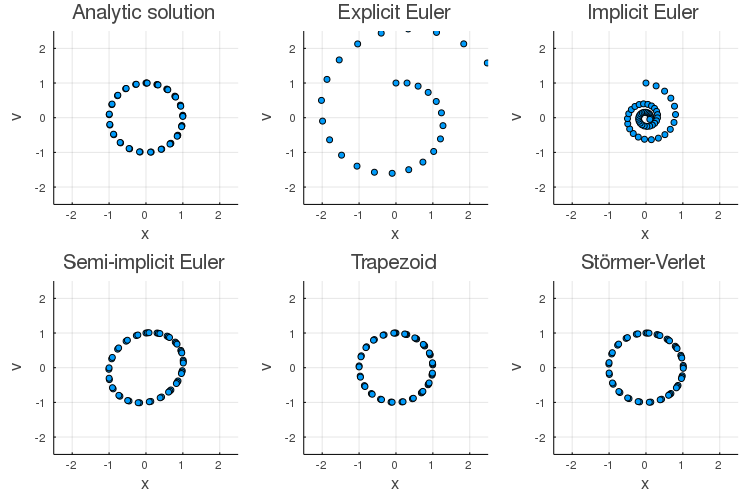
\includegraphics[width=0.85\textwidth]{stability_plots}%
  \caption{Phase space plots of the solution for the harmonic oscillator equations using different numerical methods. The angular frequency is \(\omega =1\), the total time of the simulation is 15 and the time-step is 0.3.}\label{fig:stability}%
\end{figure}

We can see a clear distinction in the solutions obtained. The trapezoid method and Störmer-Verlet method are very close to the real circular solution. On the oposite spectrum, the mplicit and explicit Euler methods show a clearly undesired behaviour, much different from the others. The semi-implicit Euler methods does a decent job, but the shape is a bit oblate. Even so, this scheme has a useful property, namely it is volume preserving. This means that the volume in phase space of the solution obtained is constant over an arbitrarily large number of periods. In contrast, the phase space volume of the implicit and explicit Euler integrators isn't even well defined because the solution diverges too fast. The difference though does not lay in volume preservence, but in what we call \textit{asimptotic stability}. The best way to study this property is mathematically. While a picture like that in~\cref{fig:stability} gives a good visual hint to what asimptotic stability of a scheme is, it was especially exagerated by choosing a large time-step. If one reruns those simulations with a time step of 0.01 instead of 0.3, almost all plots will start looking like a circle. That doesn't mean that we fixed our methods, but rather that by increasing the accuracy we made the imperfections manifest over a much larger time scale. Indeed, if we increase the total duration of the simulation enough, we would see that thing are still bad for the first two Euler methods. This is shown in~\cref{fig:stability2}.

\begin{figure}[h]
  \centering
  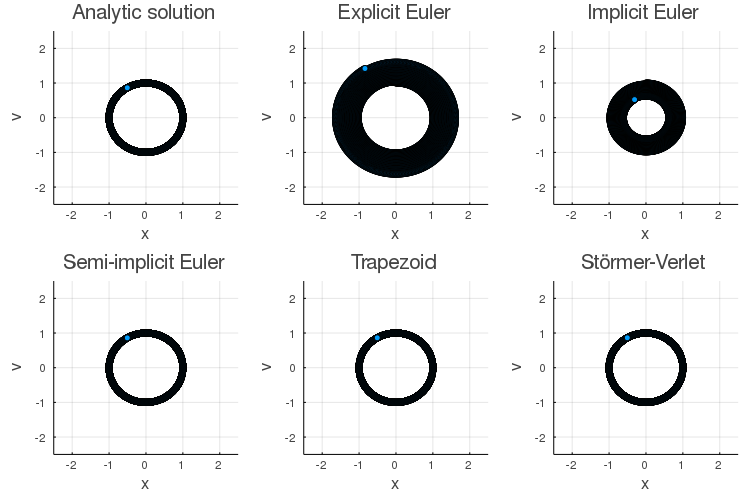
\includegraphics[width=0.85\textwidth]{stability_plots2}%
  \caption{Phase space plots of the solution for the harmonic oscillator equations using different numerical methods. The angular frequency is \(\omega =1\),  but this time around the total time of the simulation is 100 and the time-step is 0.01.}\label{fig:stability2}%
\end{figure}

\section{Methods used in Particle-in-cell simulations}
\subsection{The Boris Push}
\subsubsection{Numerical Propeties}
a
\subsection{The FDTD Maxwell Solver}
\subsubsection{Numerical Properties}
a
\subsection{FFT Based Maxwell Solvers}
a
\section{Particle-in-cell in practice}
a
\section{EPOCH}
\subsection{Software Input}
\subsection{Visualizing Results}
a
\end{document}
